\section{Rules, Values and Conventions}\label{sec:rules}

\subsection{The Board and the Moves}
We play ordinary chess, but on a different board. As usual the files are a, b, \dots, h and the ranks, from
bottom to top, are 1, \dots, 8. The cylindrical board is the $8\times 8$ board with the a-file joined to the
h-file. Only the files wrap: ranks 1 and 8 are still edges, and pawns still promote. Every piece may cross the
seam between the h- and a-files. Thus a white pawn on h4 can capture a black pawn on a5, a knight on b2 can move
to h3, and a knight on h1 gains the squares a3 and b2. A king on h1 gains a1 and a2, so a checkmate on the
ordinary board need not be a checkmate on the cylinder. A rook, bishop or queen may slide across the seam, but
it stops before its ray returns to its own square, so it cannot go round a rank as a null move. En passant
(e.p.) is allowed, including across the seam. All files are now equivalent, and there are no edge pawns. We
write $\cyl{n}$ for the cylinder with $n$ files and $\flatb{n}$ for the ordinary (flat) board with $n$ files,
both with eight ranks.

\subsection{Normal Play and the Passed-Pawn Convention}
Chess is not a normal-play game: it can be drawn, and the winner is decided by checkmate, not by who moves
last \cite{WinningWays}. Following Elkies \cite{Elkies1996}, we change it just enough to fit the theory.
\begin{itemize}
\item In pawn-only positions, a player who has no move loses. There are no null moves: a player must move on
  every turn.
\item A position in which exactly one side has a passed pawn is decided. It is worth $+\BIG$ if white has the
  passed pawn and $-\BIG$ if black has it, where $\BIG$ is larger than any count of spare moves that can arise
  (our programs use $\BIG=256$).
\item Kings are added as a group in mutual zugzwang, the tr\'ebuchet, which counts as the zero game: whoever
  has to move a king there loses a pawn, and then the game. Section~\ref{sec:kings} asks when this is exact.
\end{itemize}
So a standard win is a checkmate, while a normal-play win is a passed pawn, or an opponent with no move.

A single move, usually a capture, can give both sides a passed pawn at once. Such a promotion race needs a
rule:
\begin{itemize}
\item \emph{count}: the side that did not make the move goes first in the race; whoever needs fewer moves to
  promote wins, and a tie goes to the side that goes first;
\item \emph{mover}: the side that made the move wins;
\item \emph{opponent}: the other side wins.
\end{itemize}
None of the three is exact chess, since a new queen may give check or stop the other pawn.

\subsection{En Passant and the Passed-Pawn Test}
The convention needs a test for ``passed''. The textbook test calls a pawn passed if no enemy pawn stands ahead
of it on its own file or on a neighboring file (on the cylinder, the a- and h-files are neighbors). En passant
breaks this test. In Fig.~\ref{fig:ep_test}, white plays a2--a4. No black pawn now stands ahead of the a-pawn on
the a- or b-file, so the textbook test calls it passed. But black can answer b4$\times$a3 en passant, and the
``passed'' pawn is gone. So we use a stricter test.

\begin{figure}[!t]
\centering
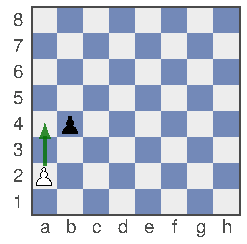
\includegraphics[width=0.42\columnwidth]{figures/ep_test.pdf}
\caption{White a2 against black b4 (ordinary board), value $0$. After a2--a4 (arrow) no black pawn stands ahead
of the a-pawn, but black may capture it en passant, b4$\times$a3, so under Definition~\ref{def:epaware} it is
not passed.}
\label{fig:ep_test}
\end{figure}

\begin{definition}[E.p.-aware passed pawn]\label{def:epaware}
A pawn is \emph{passed} if no enemy pawn stands ahead of it on its own file or a neighboring file,
\emph{and} it cannot be captured en passant on the opponent's next move, that is, it has not just made a
double step to a square beside an enemy pawn.
\end{definition}

With one more white pawn the difference decides the game. In \pos{W a2 b3 / B b4}, black has no move. The
textbook test says that white wins at once with a2--a4. Under Definition~\ref{def:epaware}, every white move
lets black capture on a3, directly after a2--a3 and en passant after a2--a4, and win the promotion race that
follows under the count rule. So the second player wins, and the value is $0$. Across the flat census of
Section~\ref{sec:atlas}, every position with at most six pawns on boards of width at most four, the stricter
test changes $21{,}441$ of the $231{,}071$ values, $4{,}068$ of them in outcome \lab{C1}.

The three race rules and three treatments of en passant (the textbook test, the e.p.-aware test, and e.p.\
off) give nine \emph{settings}. Our default setting is the count rule with the e.p.-aware test; every value
uses it unless we say otherwise.

\subsection{Components and the Cut Lemma}
A pawn changes file only when it captures, and it can only capture onto a file where an enemy pawn already
stands (en passant included). So an empty file stays empty forever, and the pawns on either side of it never
interact. Each block of neighboring occupied files is therefore a game of its own, a \emph{component}, and a
position is the sum of its components. On the ordinary board the components are blocks of adjacent files. On
the cylinder they are arcs, or one \emph{ring} that uses every file.

\begin{theorem}[Cut lemma; \lab{P}, \lab{C2}]\label{thm:cut}
A pawn position on $\cyl{n}$ with at least one empty file has the same value as the position on
$\flatb{n-1}$ obtained by cutting the cylinder open along that file.
\end{theorem}

\begin{proof}
No pawn can ever move onto the empty file, so no move ever crosses it. Cutting the board there changes no legal
move, no en passant right and no passed-pawn test, because the files beside the cut lose only a neighbor that
stays empty forever.
\end{proof}

Hence values that only a cylinder can make must come from rings (Section~\ref{sec:atlas}).
Section~\ref{sec:sums-hss} gives the condition under which a sum of components still names the right winner.

\subsection{Notation}
We write $G=\game{G^L}{G^R}$ when white (Left) can move to the positions $G^L$ and black (Right) to the
positions $G^R$, and $G+H$ for the sum in which the player to move chooses one component
\cite{WinningWays,ONAG,Siegel2013}. Every finite game has a unique \emph{canonical form}, obtained by deleting
dominated options and bypassing reversible ones, and $G=H$ exactly when $G-H$ is a second-player win. The
\emph{outcome class} of $G$ is $\mathcal{L}$ if white wins whoever starts, $\mathcal{R}$ if black does,
$\mathcal{N}$ if the first player wins and $\mathcal{P}$ if the second player wins. Our values are
\emph{numbers} (integers and dyadic fractions such as $1/2=\game{0}{1}$), \emph{nimbers}
($\star=\game{0}{0}$ and $\nim{2}=\game{0,\star}{0,\star}$), \emph{ups} (${\uparrow}=\game{0}{\star}$,
${\Uparrow}={\uparrow}+{\uparrow}$ and ${\downarrow}=-{\uparrow}$), \emph{up-second} $\upsec=\game{0}{{\downarrow}\star}$,
\emph{tinies} $\tinyg{x}=\ggame{0}{0\mid -x}$ and \emph{switches} $\pm x=\game{x}{-x}$, with
$a\pm x=\game{a+x}{a-x}$. A sum of such values is written without the plus sign, as in
${\Uparrow}\star={\Uparrow}+\star$. The \emph{birthday} of a game is the height of its canonical game tree, so
$\nim{k}$ has birthday $k$. Each game has a \emph{mean} and a \emph{temperature}, read from its thermograph
\cite{WinningWays}. The temperature measures how much the player to move gains by moving first; $\pm x$ has
temperature $x$. Infinitesimals such as $\star$, ${\uparrow}$ and $\tinyg{1}$ have mean and temperature $0$, yet
they still decide sums. The \emph{left} and \emph{right stops} of $G$ are the numbers reached when white or black
moves first and both sides play until a number appears; both stops of $0$ and of $\nim{2}$ are $0$.
